\documentclass{article}
\usepackage{lib/setup}
\usepackage{hyperref}
\addbibresource{mybibliography.bib}


%%%%%%%%%%%%%%%%%%%%%%%%%%%%%%%%%%%%%%%%%%%%%%%%%%%%%%%%%%%%%%%%%%%%%%%%%%%%%%%%
%%%%%%%%%%%%%%%%%%%%%%%%%%%%%%%%%%%%%%%%%%%%%%%%%%%%%%%%%%%%%%%%%%%%%%%%%%%%%%%%
%%%%%%%%%%%%%%%%%%%%%%%%%%%%%%%%%%%%%%%%%%%%%%%%%%%%%%%%%%%%%%%%%%%%%%%%%%%%%%%%
% Set up your information
%%%%%%%%%%%%%%%%%%%%%%%%%%%%%%%%%%%%%%%%%%%%%%%%%%%%%%%%%%%%%%%%%%%%%%%%%%%%%%%%
\subtitle{Datapath}
\title{The Shell CPU}
\author{Jonathan Rice Shelley II}
\date{\today}
\headerTitle{Shell CPU Datapath}
\subject{Version 1.0}

%%%%%%%%%%%%%%%%%%%%%%%%%%%%%%%%%%%%%%%%%%%%%%%%%%%%%%%%%%%%%%%%%%%%%%%%%%%%%%%%
%%%%%%%%%%%%%%%%%%%%%%%%%%%%%%%%%%%%%%%%%%%%%%%%%%%%%%%%%%%%%%%%%%%%%%%%%%%%%%%%
%%%%%%%%%%%%%%%%%%%%%%%%%%%%%%%%%%%%%%%%%%%%%%%%%%%%%%%%%%%%%%%%%%%%%%%%%%%%%%%%


% BEGIN DOCUMENT
\begin{document}
\maketitle

\section{Contents}
\begin{par}
	\begin{enumerate}
	\item \nameref{overview}
	\item \nameref{compd}
	\item \nameref{drt}
	\item \nameref{CPU_CTRL}
	\item \nameref{destrad}
	\end{enumerate}
\end{par}

\section{Shell Datapath Overview}
\label{overview}
\begin{par}
	The Shell datapath is shown in full in figure 4. The CPUs system memory is based on the Harvard architecture separating data and program memory (Figure 1 and 2). In figure 3 the CPU is shown without the surrounding memory. A high resolution picture of the full datapath can be found at this \href{https://raw.githubusercontent.com/RiceShelley/ELEC-5200/master/blockD.png}{link}.
	
	\begin{figure}[H]
		\centering
		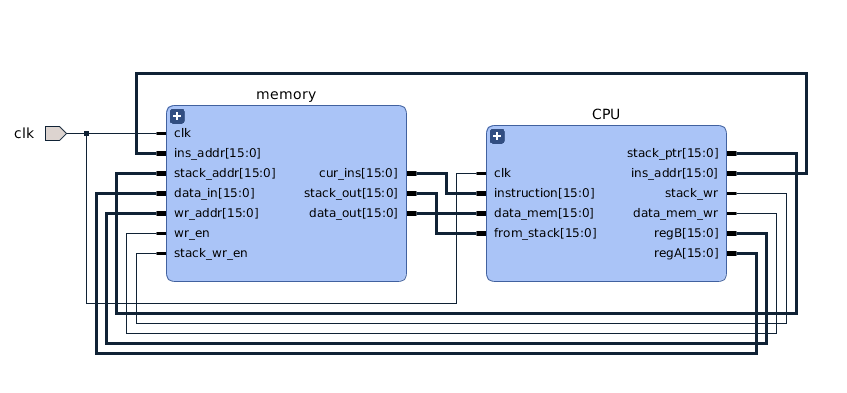
\includegraphics[width=5in]{img/system_ov.png}
		\caption{Top level separation of CPU and memory.}
	\end{figure}

		\begin{figure}[H]
		\centering
		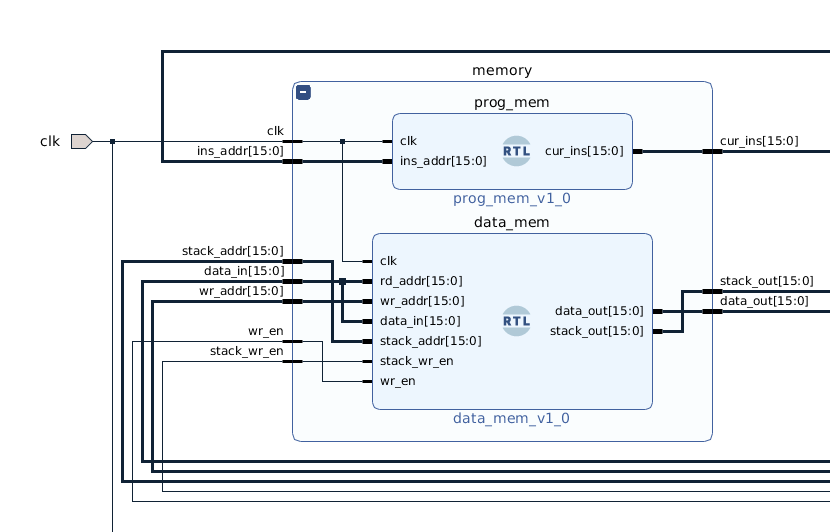
\includegraphics[width=6in]{img/sysmem.png}
		\caption{System memory.}
	\end{figure}
	
	\hspace{100pt}
	
	\begin{figure}[H]
		\centering
		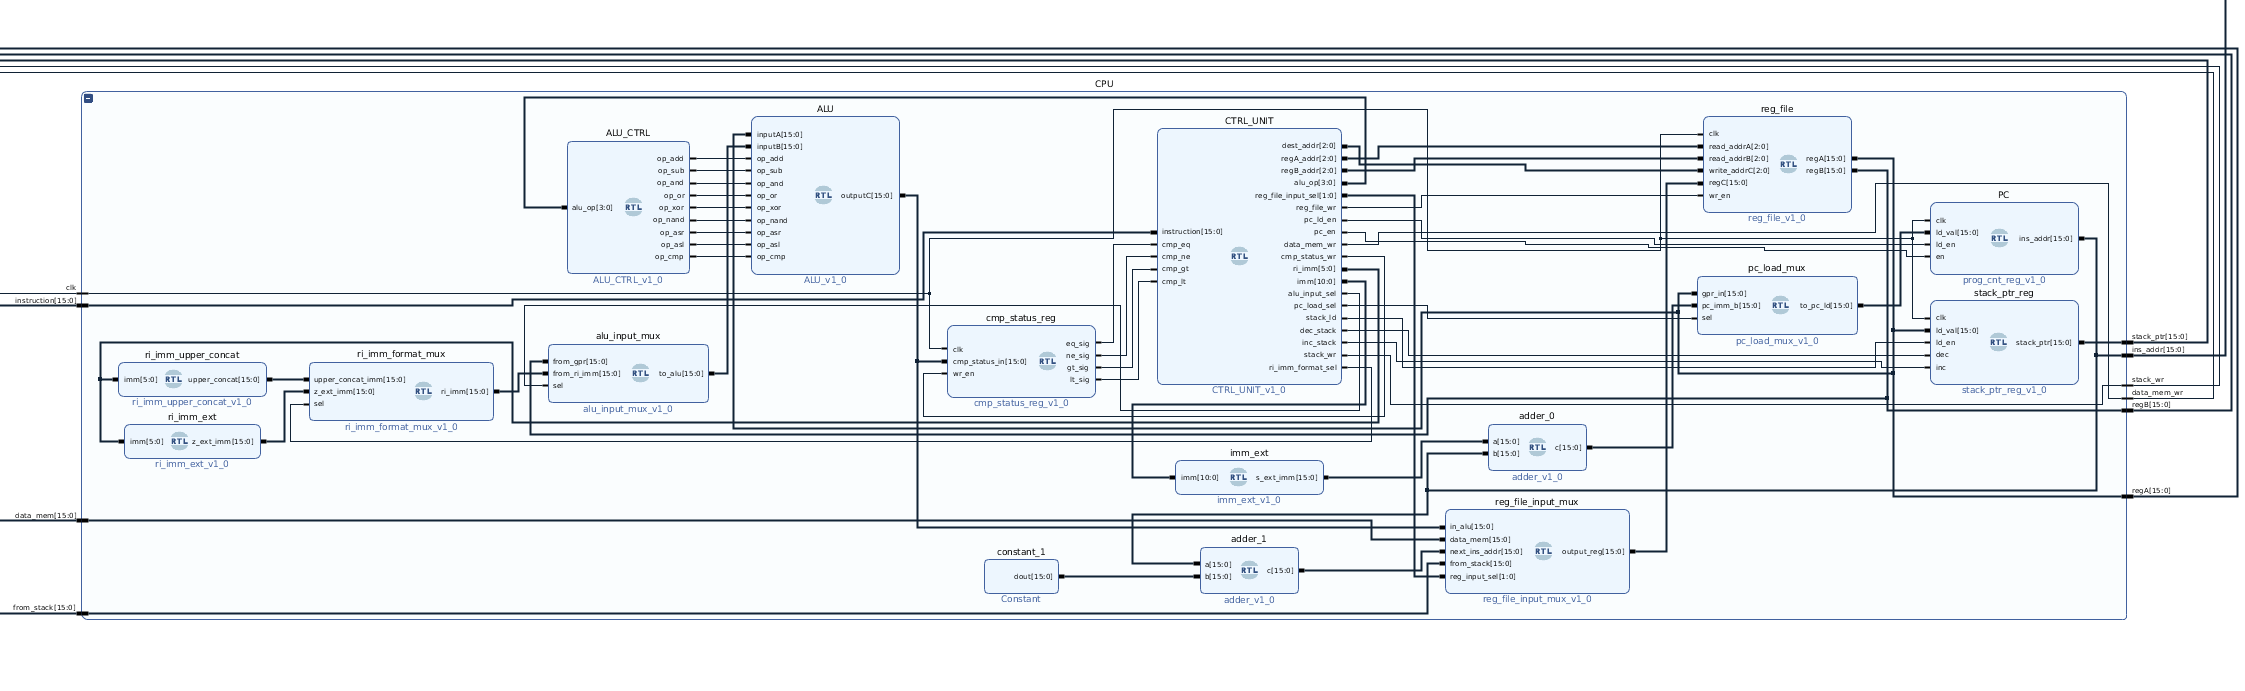
\includegraphics[width=7in]{img/cpuov.png}
		\caption{CPU structure.}
	\end{figure}

	\begin{figure}[H]
		\centering
		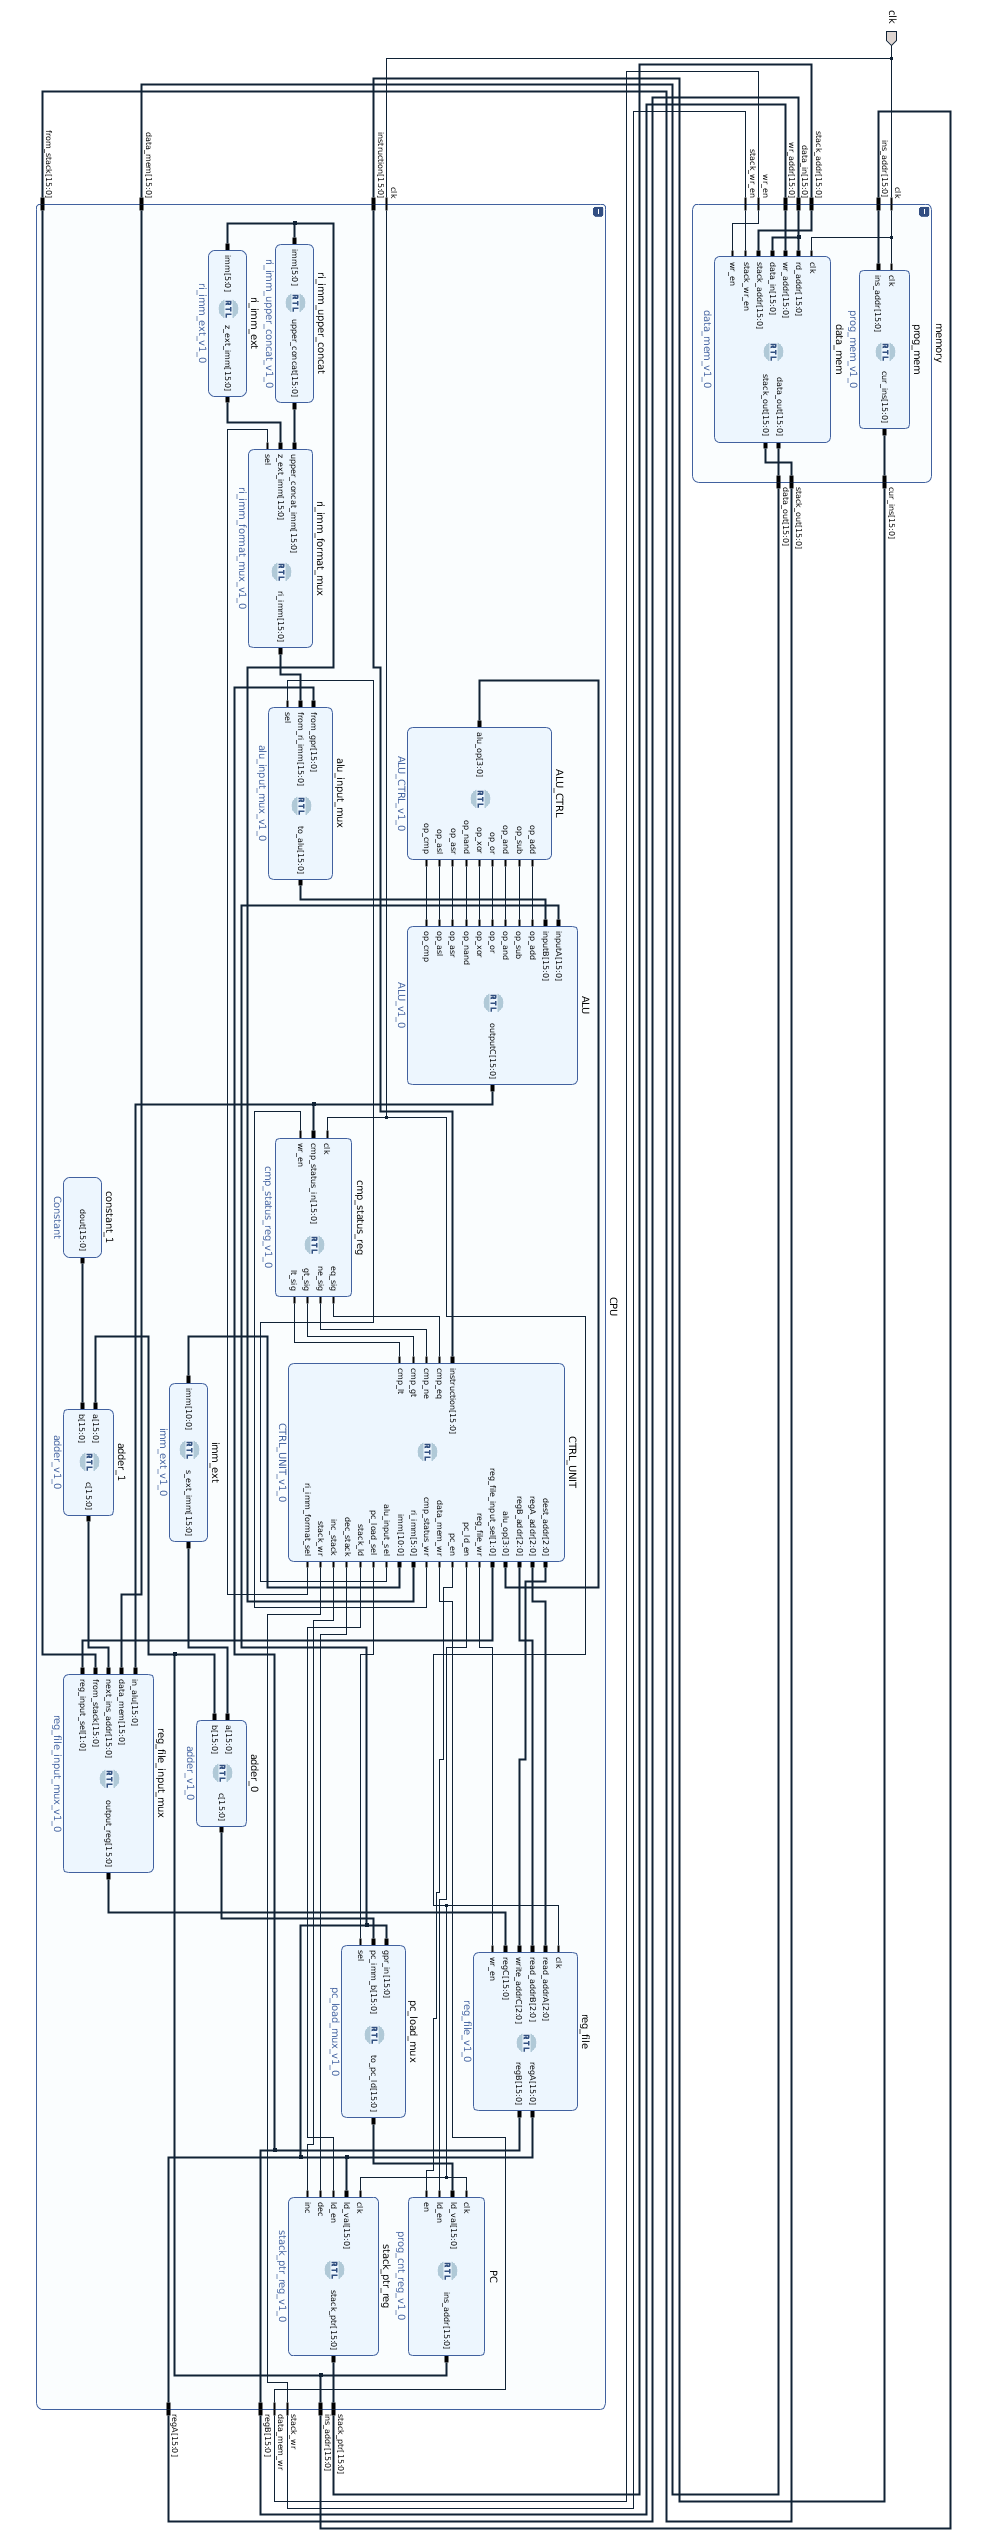
\includegraphics[width=3.5in]{img/dsf.png}
		\caption{Full CPU structure (rotated for increased resolution).}
	\end{figure}
	
\end{par}

\newpage

\section{Component Descriptions}
\label{compd}
\begin{par}
	
	Description of inputs, outputs, and function of each component in the datapath. 
	
	\subsection{Arithmetic Logic Unit}
	
	\begin{figure}[H]
		\centering
		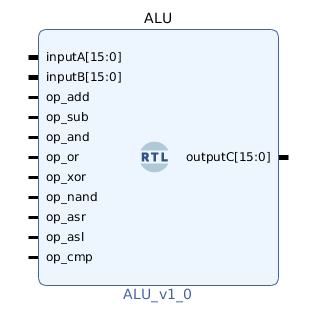
\includegraphics[width=2in]{img/alu.png}
		\caption{Arithmetic Logic Unit}
	\end{figure}

	\textbf{Functional description}
	\begin{par}
		The arithmetic logic unit or ALU performs arithmetic operations on data in the CPU. The block is entirely combinational logic and controlled by its "op" signals. ALU op code signals are one hot. In the event that multiple signals are high priority will be taken to the op code signal that appears first in the IO table below.  
	\end{par}
	
	\begin{center}
		\begin{tabular}{|c|c|}
			\hline 
			\multicolumn{2}{|c|}{\textbf{IO table}} \\
			\hline 
			\textbf{Inputs} & \textbf{Description} \\ 
			\hline 
			inputA & 16 bit bus, ALU operand \\ 
			\hline 
			inputB & 16 bit bus, 2nd ALU operand \\
			\hline
			op\_add & if signal high add operands \\
			\hline
			op\_sub & if signal high subtract operands \\
			\hline
			op\_and & if signal high bit-wise and operands \\
			\hline
			op\_or & if signal high bit-wise or operands \\
			\hline
			op\_xor & if signal high bit-wise xor operands \\
			\hline
			op\_nand & if signal high bit-wise nand operands \\
			\hline
			op\_asr & if signal high arithmetic shift 1 bit right input A \\
			\hline
			op\_asl & if signal high arithmetic shift 1 bit left input A \\
			\hline
			op\_cmp & if signal high compare operands. \\
			\hline
			\textbf{Outputs} & \textbf{Description} \\ 
			\hline 
			outputC & the 16 bit result of some operation on input A and B \\
			\hline
		\end{tabular} 
	\end{center}

	\subsection{Simple Adder}
	
	\begin{figure}[H]
		\centering
		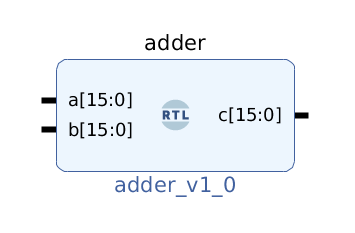
\includegraphics[width=2in]{img/simpleAddr.png}
		\caption{Simple adder unit}
	\end{figure}
	
	\textbf{Functional description}
	\begin{par}
		The simple adder block is used to sum values together within the CPU datapath. The block is used once to calculate PC + 1. The block is used a second time to find pc + imm for B-Type instructions. 
	\end{par}
	
	\begin{center}
		\begin{tabular}{|c|c|}
			\hline 
			\multicolumn{2}{|c|}{\textbf{IO table}} \\
			\hline 
			\textbf{Inputs} & \textbf{Description} \\ 
			\hline 
			a & 16 bit bus \\ 
			\hline 
			b & 16 bit bus \\ 
			\hline 
			\textbf{Outputs} & \textbf{Description} \\ 
			\hline 
			c & 16 bit bus, assigned to sum of a and b. \\ 
			\hline 
		\end{tabular} 
	\end{center}

	\newpage

	\subsection{Arithmetic Logic Unit Controller}
	
	\begin{figure}[H]
		\centering
		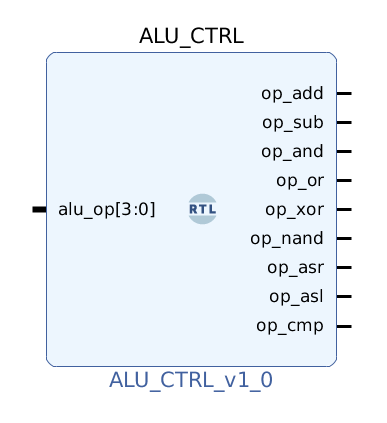
\includegraphics[width=2in]{img/aluCtrl.png}
		\caption{Arithmetic Logic Unit Controller}
	\end{figure}

	\textbf{Functional description}
	\begin{par}
		The arithmetic logic unit controller is used to interpret the ALU op codes from the CPU controller. The outputs of the arithmetic logic unit controller directly control what operation the ALU performs. 
	\end{par}
	
	\begin{center}
		\begin{tabular}{|c|c|}
			\hline 
			\multicolumn{2}{|c|}{\textbf{IO table}} \\
			\hline 
			\textbf{Inputs} & \textbf{Description} \\ 
			\hline 
			alu\_op & ALU op code from CPU controller \\ 
			\hline 
			\textbf{Outputs} & \textbf{Description} \\ 
			\hline 
			op\_add & add operands \\
			\hline
			op\_sub & subtract operands \\
			\hline
			op\_and & bit-wise and operands \\
			\hline
			op\_or & bit-wise or operands \\
			\hline
			op\_xor & bit-wise xor operands \\
			\hline
			op\_nand & bit-wise nand operands \\
			\hline
			op\_asr & arithmetic shift 1 bit right input A \\
			\hline
			op\_asl & arithmetic shift 1 bit left input A \\
			\hline
			op\_cmp & compare operands. \\
			\hline
		\end{tabular} 
	\end{center}

	\newpage
	
	\subsection{Arithmetic Logic Unit Input Multiplexer}
	
	\begin{figure}[H]
		\centering
		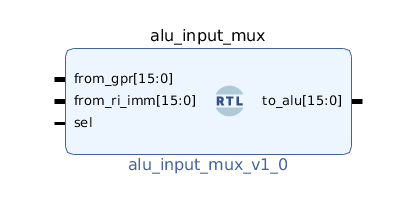
\includegraphics[width=1.5in]{img/aluMux.png}
		\caption{Arithmetic Logic Unit Input Multiplexer}
	\end{figure}
	
	\textbf{Functional description}
	\begin{par}
		The arithmetic logic unit input multiplexer is used to mux the input to the 16-bit B operand of the ALU. The input to the ALU can be switched between the output of the GPR file or a ri\_imm.
	\end{par}
	
	\begin{center}
		\begin{tabular}{|c|c|}
			\hline 
			\multicolumn{2}{|c|}{\textbf{IO table}} \\
			\hline 
			\textbf{Inputs} & \textbf{Description} \\ 
			\hline 
			from\_gpr & 16-bit input from GPR file \\ 
			\hline 
			from\_ri\_imm & 16-bit input from ri\_imm \\ 
			\hline 
			sel & select line of multiplexer \\ 
			\hline 
			\textbf{Outputs} & \textbf{Description} \\ 
			\hline 
			to\_alu & 16-bit output of mux \\
			\hline
		\end{tabular} 
	\end{center}

	\subsection{Comparator Status Register}
	
	\begin{figure}[H]
		\centering
		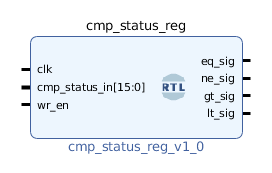
\includegraphics[width=1.5in]{img/cmpStat.png}
		\caption{Comparator Status Register}
	\end{figure}
	
	\textbf{Functional description}
	\begin{par}
		The comparator status register stores the results of a comparison. 
	\end{par}
	
	\begin{center}
		\begin{tabular}{|c|c|}
			\hline 
			\multicolumn{2}{|c|}{\textbf{IO table}} \\
			\hline 
			\textbf{Inputs} & \textbf{Description} \\ 
			\hline 
			clk & CPU clk signal \\ 
			\hline 
			cmp\_status\_in & 16-bit result of comparison from ALU \\ 
			\hline 
			wr\_en & write enable line \\ 
			\hline 
			\textbf{Outputs} & \textbf{Description} \\ 
			\hline 
			eq\_sig & High when comparison shows equality \\
			\hline
			ne\_sig & High when comparison shows inequality \\
			\hline
			gt\_sig & High when comparison is greater than \\
			\hline
			lt\_sig & High when comparison is less than \\
			\hline
		\end{tabular} 
	\end{center}
	
	\newpage
	
	\subsection{CPU Control Unit}
	
	\begin{figure}[H]
		\centering
		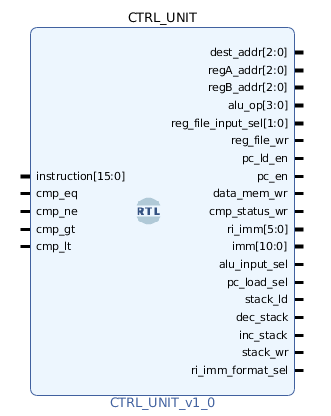
\includegraphics[width=1.2in]{img/ctrlUnit.png}
		\caption{CPU Control Unit}
	\end{figure}
	
	\textbf{Functional description}
	\begin{par}
		The CPU control unit decodes instructions and configures the CPU to execute the instructions. 
	\end{par}
	
	\begin{center}
		\begin{tabular}{|c|c|}
			\hline 
			\multicolumn{2}{|c|}{\textbf{IO table}} \\
			\hline 
			\textbf{Inputs} & \textbf{Description} \\ 
			\hline 
			instruction & 16-bit instruction \\ 
			\hline 
			cmp\_eq & status bit from last comparison \\ 
			\hline 
			cmp\_ne & status bit from last comparison \\ 
			\hline 
			cmp\_gt & status bit from last comparison \\ 
			\hline 
			cmp\_lt & status bit from last comparison \\ 
			\hline 
			\textbf{Outputs} & \textbf{Description} \\ 
			\hline 
			dest\_addr & Address of destination register \\
			\hline
			regA\_addr & Address of register A \\
			\hline
			regB\_addr & Address of register B \\
			\hline
			alu\_op & ALU op code \\
			\hline
			reg\_file\_input\_sel & select line for reg file input mux \\
			\hline
			reg\_file\_wr & register file write line \\ 
			\hline 
			pc\_ld\_en & load PC reg enable line \\ 
			\hline 
			pc\_en & enable PC increment signal \\ 
			\hline 
			data\_mem\_wr & write to data memory signal \\ 
			\hline 
			cmp\_status\_wr & write to comparator register signal \\ 
			\hline 
			ri\_imm[5:0] & ri-type 6-bit immediate \\ 
			\hline 
			imm[10:0] & B-type 11 bit immediate \\ 
			\hline 
			alu\_input\_sel & ALU input mux select line \\ 
			\hline 
			pc\_load\_sel & program counter load input mux select line \\ 
			\hline 
			stack\_ld & stack load input signal \\ 
			\hline 
			dec\_stack & decrement stack input signal \\ 
			\hline 
			inc\_stack & increment stack input signal \\ 
			\hline 
			stack\_wr & enable writing to memory at stack pointer \\ 
			\hline 
			ri\_imm\_format\_sel & ri-type format mux select line \\ 
			\hline 
		\end{tabular} 
	\end{center}
	
	\newpage
	
	\subsection{Data Memory}
	
	\begin{figure}[H]
		\centering
		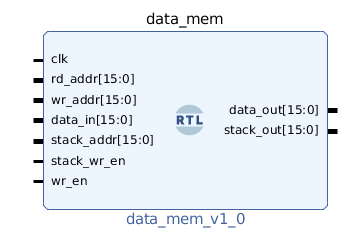
\includegraphics[width=1.5in]{img/dataMem.png}
		\caption{Data Memory}
	\end{figure}

	\textbf{Functional description}
	\begin{par}
		Memory for stack and program data. 
	\end{par}
	
	\begin{center}
		\begin{tabular}{|c|c|}
			\hline 
			\multicolumn{2}{|c|}{\textbf{IO table}} \\
			\hline 
			\textbf{Inputs} & \textbf{Description} \\ 
			\hline 
			clk & CPU clk signal \\ 
			\hline 
			rd\_addr & 16-bit read address \\ 
			\hline 
			wr\_addr & 16-bit write address \\ 
			\hline 
			data\_in & 16-bit word to write \\ 
			\hline 
			stack\_addr & 16-bit stack pointer \\ 
			\hline 
			stack\_wr\_en & stack write enable \\ 
			\hline 
			wr\_en & memory write enable \\ 
			\hline 
			\textbf{Outputs} & \textbf{Description} \\ 
			\hline 
			data\_out & 16-bit word from memory at wr\_addr \\
			\hline
			stack\_out & 16-bit word from memory at stack pointer \\
			\hline
		\end{tabular} 
	\end{center}

	\subsection{11-bit Immediate Sign Extend}
	
	\begin{figure}[H]
		\centering
		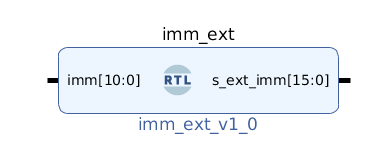
\includegraphics[width=2in]{img/immExt.png}
		\caption{11-bit Immediate Sign Extend}
	\end{figure}
	
	\textbf{Functional description}
	\begin{par}
		Used to sign extend 11-bit immediates from B-type instructions.  
	\end{par}
	
	\begin{center}
		\begin{tabular}{|c|c|}
			\hline 
			\multicolumn{2}{|c|}{\textbf{IO table}} \\
			\hline 
			\textbf{Inputs} & \textbf{Description} \\ 
			\hline 
			imm & immediate from b-type instruction \\ 
			\hline 
			\textbf{Outputs} & \textbf{Description} \\ 
			\hline 
			s\_ext\_imm & sign extended immediate from b-type instruction \\
			\hline
		\end{tabular} 
	\end{center}

	\newpage

	\subsection{Program Counter Load Multiplexer}
	
	\begin{figure}[H]
		\centering
		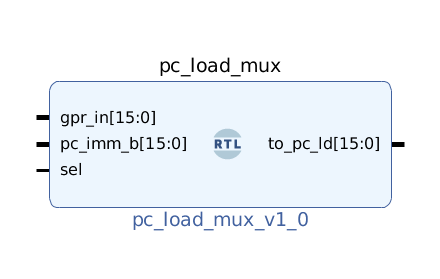
\includegraphics[width=2in]{img/pclmux.png}
		\caption{Program Counter Load Multiplexer}
	\end{figure}
	
	\textbf{Functional description}
	\begin{par}
		Used to multiplex inputs to PC load bus.
	\end{par} 
	
	\begin{center}
		\begin{tabular}{|c|c|}
			\hline 
			\multicolumn{2}{|c|}{\textbf{IO table}} \\
			\hline 
			\textbf{Inputs} & \textbf{Description} \\ 
			\hline 
			gpr\_in & GPR file 16-bit output \\ 
			\hline 
			pc\_imm\_b & value of pc + immediate \\ 
			\hline 
			sel & multiplexer select signal \\ 
			\hline 
			\textbf{Outputs} & \textbf{Description} \\ 
			\hline 
			to\_pc\_ld & output value to PC load word port \\
			\hline
		\end{tabular} 
	\end{center}
	
	\subsection{Program Counter Register}
	
	\begin{figure}[H]
		\centering
		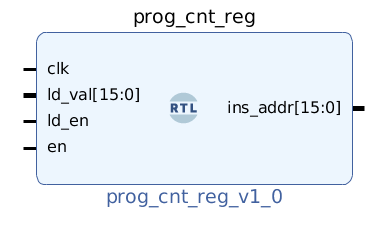
\includegraphics[width=2in]{img/progCnt.png}
		\caption{Program Counter Register}
	\end{figure}
	
	\textbf{Functional description}
	\begin{par}
		Program counter used to keep the address of the next instruction in memory. 
	\end{par}
	
	\begin{center}
		\begin{tabular}{|c|c|}
			\hline 
			\multicolumn{2}{|c|}{\textbf{IO table}} \\
			\hline 
			\textbf{Inputs} & \textbf{Description} \\ 
			\hline 
			clk & CPU clock \\ 
			\hline 
			ld\_val & 16-bit word to load PC with \\ 
			\hline 
			ld\_en & PC load enable \\ 
			\hline 
			en & enable PC increment. \\ 
			\hline 
			\textbf{Outputs} & \textbf{Description} \\ 
			\hline 
			ins\_addr & address of the next instruction in memory \\
			\hline
		\end{tabular}
	\end{center}

	\subsection{Program Memory}
	
	\begin{figure}[H]
		\centering
		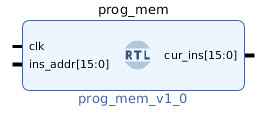
\includegraphics[width=2in]{img/progMem.png}
		\caption{Program Memory}
	\end{figure}
	
	\textbf{Functional description}
	\begin{par}
		Program memory used to store program instructions. 
	\end{par}
	
	\begin{center}
		\begin{tabular}{|c|c|}
			\hline 
			\multicolumn{2}{|c|}{\textbf{IO table}} \\
			\hline 
			\textbf{Inputs} & \textbf{Description} \\ 
			\hline 
			clk & CPU clock \\ 
			\hline 
			ins\_addr & instruction address \\ 
			\hline 
			\textbf{Outputs} & \textbf{Description} \\ 
			\hline 
			cur\_ins & current instruction \\
			\hline
		\end{tabular}
	\end{center}

	\subsection{General Purpose Register File}
	
	\begin{figure}[H]
		\centering
		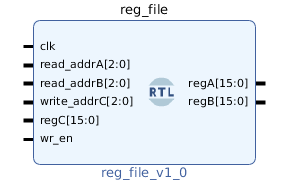
\includegraphics[width=1.6in]{img/regFile.png}
		\caption{General Purpose Register File}
	\end{figure}
	
	\textbf{Functional description}
	\begin{par}
		GPR (General Purpose Register) file is used to store temporary values during computation.
	\end{par} 
	
	\begin{center}
		\begin{tabular}{|c|c|}
			\hline 
			\multicolumn{2}{|c|}{\textbf{IO table}} \\
			\hline 
			\textbf{Inputs} & \textbf{Description} \\ 
			\hline 
			clk & CPU clock \\ 
			\hline 
			read\_addrA & GPR address \\ 
			\hline 
			read\_addrB & GPR address \\ 
			\hline 
			write\_addrC & GPR address \\ 
			\hline 
			regC & data word to be written to GPR \\ 
			\hline 
			wr\_en & write enable \\ 
			\hline 
			\textbf{Outputs} & \textbf{Description} \\ 
			\hline 
			regA & contents of GPR at addrA \\
			\hline
			regB & contents of GPR at addrB \\
			\hline
		\end{tabular}
	\end{center}

	\newpage
	
	\subsection{Register File Input Multiplexer}
	
	\begin{figure}[H]
		\centering
		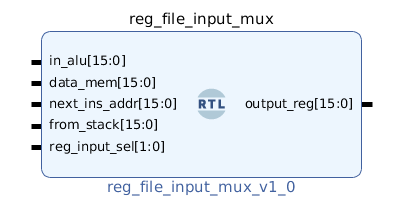
\includegraphics[width=2in]{img/regFileMux.png}
		\caption{Register File Input Multiplexer}
	\end{figure}
	
	\textbf{Functional description}
	\begin{par}
		Used to multiplex the data input to the GPR file. 
	\end{par}
	
	\begin{center}
		\begin{tabular}{|c|c|}
			\hline 
			\multicolumn{2}{|c|}{\textbf{IO table}} \\
			\hline 
			\textbf{Inputs} & \textbf{Description} \\ 
			\hline 
			in\_alu & 16-bit output from ALU \\ 
			\hline 
			data\_mem & 16-bit output from data memory \\ 
			\hline 
			next\_ins\_addr & 16-bit PC + 1 \\ 
			\hline 
			from\_stack & 16-bit word from stack \\ 
			\hline 
			reg\_input\_sel & multiplexer select line \\ 
			\hline 
			\textbf{Outputs} & \textbf{Description} \\ 
			\hline 
			output\_reg & 16-bit output of multiplexer \\
			\hline
		\end{tabular}
	\end{center}

	\subsection{RI-Type Zero Extend Immediate}
	
	\begin{figure}[H]
		\centering
		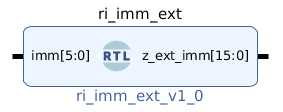
\includegraphics[width=2in]{img/riImmExt.png}
		\caption{RI-Type Zero Extend Immediate}
	\end{figure}
	
	\textbf{Functional description}
	\begin{par}
		Used to zero extend the ri-type immediate field. 
	\end{par}
	
	\begin{center}
		\begin{tabular}{|c|c|}
			\hline 
			\multicolumn{2}{|c|}{\textbf{IO table}} \\
			\hline 
			\textbf{Inputs} & \textbf{Description} \\ 
			\hline 
			imm & 6-bit immediate \\ 
			\hline 
			\textbf{Outputs} & \textbf{Description} \\ 
			\hline 
			z\_ext\_imm & 16-bit zero extended 6-bit immediate \\
			\hline
		\end{tabular}
	\end{center}

	\newpage
	
	\subsection{RI-Type Immediate Format Multiplexer}
	
	\begin{figure}[H]
		\centering
		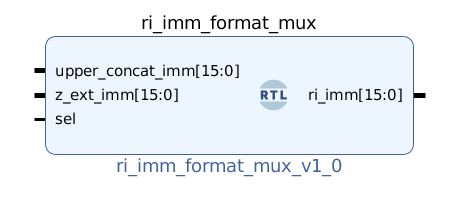
\includegraphics[width=2in]{img/riImmF.png}
		\caption{RI-Type Immediate Format Multiplexer}
	\end{figure}
	
	\textbf{Functional description}
	\begin{par}
		Multiplex RI-Type immediate between zero extended and upper 6-bit concatenation format. 
	\end{par}
	
	\begin{center}
		\begin{tabular}{|c|c|}
			\hline 
			\multicolumn{2}{|c|}{\textbf{IO table}} \\
			\hline 
			\textbf{Inputs} & \textbf{Description} \\ 
			\hline 
			upper\_concat\_imm & 16-bit concat immediate \\ 
			\hline 
			z\_ext\_imm & 16-bit zero extended immediate \\ 
			\hline 
			sel & multiplexer select line \\ 
			\hline 
			\textbf{Outputs} & \textbf{Description} \\ 
			\hline 
			ri\_imm & 16-bit formatted ri-type immediate \\
			\hline
		\end{tabular}
	\end{center}

	\subsection{RI-Type Immediate Upper 6-bit Concatenation}
	
	\begin{figure}[H]
		\centering
		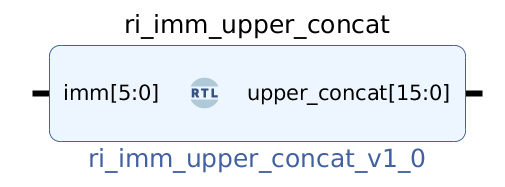
\includegraphics[width=2in]{img/upcon.png}
		\caption{RI-Type Immediate Upper 6-bit Concatenation}
	\end{figure}
	
	\textbf{Functional description}
	\begin{par}
		Concatenate 6-bit immediate with upper part of 16-bit register zero all lower bits. 
	\end{par}
	
	\begin{center}
		\begin{tabular}{|c|c|}
			\hline 
			\multicolumn{2}{|c|}{\textbf{IO table}} \\
			\hline 
			\textbf{Inputs} & \textbf{Description} \\ 
			\hline 
			imm & 6-bit immediate \\ 
			\hline 
			\textbf{Outputs} & \textbf{Description} \\ 
			\hline 
			upper\_concat & 16-bit formatted ri-type immediate \\
			\hline
		\end{tabular}
	\end{center}

	\newpage
	
	\subsection{Stack Pointer Register}
	
	\begin{figure}[H]
		\centering
		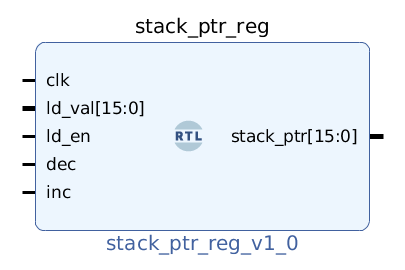
\includegraphics[width=2in]{img/stackPtr.png}
		\caption{Stack Pointer Register}
	\end{figure}

	\textbf{Functional description}
	\begin{par}
		Register holds stack pointer. 
	\end{par}
	
	\begin{center}
		\begin{tabular}{|c|c|}
			\hline 
			\multicolumn{2}{|c|}{\textbf{IO table}} \\
			\hline 
			\textbf{Inputs} & \textbf{Description} \\ 
			\hline 
			clk & CPU clk \\ 
			\hline 
			ld\_val & word to be loaded into stack pointer \\ 
			\hline 
			ld\_en & enable write to stack pointer register \\ 
			\hline 
			dec & decrement stack pointer \\ 
			\hline 
			inc & increment stack pointer \\ 
			\hline 
			\textbf{Outputs} & \textbf{Description} \\ 
			\hline 
			stack\_ptr & 16-bit stack pointer \\
			\hline
		\end{tabular}
	\end{center}

\end{par}

\newpage

\section{Datapath Register Transfers}
\label{drt}
\begin{par}
	
	The datapath register transfers section details the register transfers that take place for each instruction. In the below table $ R_{n} $ corresponds to registers in the GPR file. 
	
	\begin{center}
		\begin{tabular}{|c|c|c|}
			\hline
			\textbf{No.} & \textbf{Instruction} & \textbf{Register Transfers} \\
			\hline 
			1 & hlt & PC $ => $ PC \\
			\hline 
			2 & add $ R_{1} $, $ R_{2} $, $ R_{3} $ & $ R_{2} $, $ R_{3} $ $ => $ ALU $ => $ $ R_{3} $ \\
			\hline
			3 & sub $ R_{1} $, $ R_{2} $, $ R_{3} $ & $ R_{2} $, $ R_{3} $ $ => $ ALU $ => $ $ R_{3} $ \\
			\hline
			4 & and $ R_{1} $, $ R_{2} $, $ R_{3} $ & $ R_{2} $, $ R_{3} $ $ => $ ALU $ => $ $ R_{3} $ \\
			\hline
			5 & or $ R_{1} $, $ R_{2} $, $ R_{3} $ & $ R_{2} $, $ R_{3} $ $ => $ ALU $ => $ $ R_{3} $ \\
			\hline
			6 & xor $ R_{1} $, $ R_{2} $, $ R_{3} $ & $ R_{2} $, $ R_{3} $ $ => $ ALU $ => $ $ R_{3} $ \\
			\hline
			7 & nand $ R_{1} $, $ R_{2} $, $ R_{3} $ & $ R_{2} $, $ R_{3} $ $ => $ ALU $ => $ $ R_{3} $ \\
			\hline
			8 & lw $ R_{1} $, $ R_{2} $ & $ R_{2} $ $ => $ Data Memory $ => $ $ R_{1} $ \\
			\hline
			9 & sw $ R_{1} $, $ R_{2} $ & $ R_{1} $, $ R_{2} $ $ => $ Data Memory \\
			\hline
			10 & asr $ R_{1} $, $ R_{2} $ & $ R_{2} $ $ => $ ALU $ => $ $ R_{1} $ \\
			\hline
			11 & asl $ R_{1} $, $ R_{2} $ & $ R_{2} $ $ => $ ALU $ => $ $ R_{1} $ \\
			\hline
			12 & cmp $ R_{1} $, $ R_{2} $ & $ R_{1} $, $ R_{2} $ $ => $ ALU $ => $ compare register \\
			\hline
			13 & jalr $ R_{1} $, $ R_{2} $ & PC $ => $ + 1 adder $ => $ $ R_{1} $ $ | $ $ R_{2} $ $ => $ PC \\
			\hline
			14 & push $ R_{1} $ & $ R_{1} $ $ => $ data memory at addr SP \\
			\hline
			15 & pop $ R_{1} $ & data memory at addr SP $ => $ $ R_{1} $ \\
			\hline
			16 & lsp $ R_{1} $ & $ R_{1} $ $ => $ Stack Pointer Register \\
			\hline
			17 & addi $ R_{1} $, $ imm $ &  $ R_{1} $, $ imm $ $ => $ zero extend $ => $ ALU $ => $ $ R_{1} $ \\
			\hline
			18 & subi $ R_{1} $, $ imm $ & $ R_{1} $, $ imm $ $ => $ zero extend $ => $ ALU $ => $ $ R_{1} $ \\
			\hline
			19 & lui $ R_{1} $, $ imm $ & $ R_{1} $, $ imm $ $ => $ zero extend $ => $ ALU $ => $ $ R_{1} $ \\
			\hline
			20 & beq $ imm $ & $ imm $ $ => $ sign extend $ => $ + current PC adder $ => $ PC \\
			\hline
			21 & bne $ imm $ & $ imm $ $ => $ sign extend $ => $ + current PC adder $ => $ PC \\
			\hline
			22 & bgt $ imm $ & $ imm $ $ => $ sign extend $ => $ + current PC adder $ => $ PC \\
			\hline
			23 & blt $ imm $ & $ imm $ $ => $ sign extend $ => $ + current PC adder $ => $ PC \\
			\hline
		\end{tabular}
	\end{center}
	
\end{par}
\newpage

\section{CPU Control and Operation}
\label{CPU_CTRL}
\begin{par}
	
	This section list all control signals and their values needed to perform each instruction in the Shell ISA. 

	\begin{figure}[H]
		\centering
		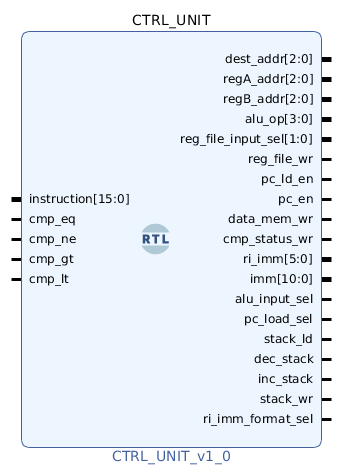
\includegraphics[width=2in]{img/ctrl_unit.png}
		\caption{Shell CPU Control Unit}
	\end{figure}

	To perform each instruction the combinational logic control unit shown above must decode the 16-bit instruction and configure its outputs to set the CPU into the desired state. Each instruction will configure the outputs of this block in a unique format. The outputs for proper control unit configuration for \textbf{every} instruction is listed below.
	
	\hspace{1pt}
	
	The key below describes the symbols used in the tables that describe the control unit output for each instruction. Each symbol will always correspond to 1 bit. 
	
	\begin{center}
		\begin{tabular}{|c|c|}
			\hline 
			\multicolumn{2}{|c|}{\textbf{Control Truth Table Symbol Key}} \\
			\hline 
			\textbf{Symbol} & \textbf{Description} \\ 
			\hline 
			0 & 0 bit / low signal \\ 
			\hline 
			1 & 1 bit / high signal \\ 
			\hline 
			x & don't care bit \\ 
			\hline 
			n & value defined by field in instruction. Ex: (imm or GPR addresses) \\ 
			\hline 
			\{ ctrl\_unit\_input\_sig\_name \} & \{\} denotes the use of a ctrl unit input signal \\ 
			\hline 
		\end{tabular} 
	\end{center}
	
	\newpage
	\subsection{Halt S-Type Instruction}
	
	The halt instruction stops the CPU from executing instructions. \\
	
	\begin{center}
		\begin{tabular}{|c|c|}
			\hline 
			\textbf{Signal} & \textbf{Binary value} \\ 
			\hline 
			dest\_addr[2:0] & xxx \\ 
			\hline 
			regA\_addr[2:0] & xxx \\ 
			\hline 
			regB\_addr[2:0] & xxx \\ 
			\hline 
			alu\_op[3:0] & xxxx \\ 
			\hline 
			reg\_file\_input\_sel[1:0] & xx \\ 
			\hline 
			reg\_file\_wr & 0 \\ 
			\hline 
			pc\_ld\_en & 0 \\ 
			\hline 
			pc\_en & 0 \\ 
			\hline 
			data\_mem\_wr & 0 \\ 
			\hline 
			cmp\_status\_wr & 0 \\ 
			\hline 
			ri\_imm[5:0] & xxxxxx \\ 
			\hline 
			imm[10:0] & xxxxxxxxxxx \\ 
			\hline 
			alu\_input\_sel & x \\ 
			\hline 
			pc\_load\_sel & x \\ 
			\hline 
			stack\_ld & 0 \\ 
			\hline 
			dec\_stack & 0 \\ 
			\hline 
			inc\_stack & 0 \\ 
			\hline 
			stack\_wr & 0 \\ 
			\hline 
			ri\_imm\_format\_sel & x \\ 
			\hline 
		\end{tabular} 
	\end{center}

	\newpage
	\subsection{Add RRR-Type Instruction}
	
	The add instruction uses the ALU to add 2 registers from the GPR file and stores the result back in the GPR file. \\
	
	\begin{center}
		\begin{tabular}{|c|c|}
			\hline 
			\textbf{Signal} & \textbf{Binary value} \\ 
			\hline 
			dest\_addr[2:0] & nnn \\ 
			\hline 
			regA\_addr[2:0] & nnn \\ 
			\hline 
			regB\_addr[2:0] & nnn \\ 
			\hline 
			alu\_op[3:0] & 0000 \\ 
			\hline 
			reg\_file\_input\_sel[1:0] & 00 \\ 
			\hline 
			reg\_file\_wr & 1 \\ 
			\hline 
			pc\_ld\_en & 0 \\ 
			\hline 
			pc\_en & 1 \\ 
			\hline 
			data\_mem\_wr & 0 \\ 
			\hline 
			cmp\_status\_wr & 0 \\ 
			\hline 
			ri\_imm[5:0] & xxxxxx \\ 
			\hline 
			imm[10:0] & xxxxxxxxxxx \\ 
			\hline 
			alu\_input\_sel & 0 \\ 
			\hline 
			pc\_load\_sel & x \\ 
			\hline 
			stack\_ld & 0 \\ 
			\hline 
			dec\_stack & 0 \\ 
			\hline 
			inc\_stack & 0 \\ 
			\hline 
			stack\_wr & 0 \\ 
			\hline 
			ri\_imm\_format\_sel & x \\ 
			\hline 
		\end{tabular} 
	\end{center}

	\newpage
	\subsection{Sub RRR-Type Instruction}
	
	The sub instruction uses the ALU to subtract 2 registers from the GPR file and stores the result back in the GPR file. \\
	
	\begin{center}
		\begin{tabular}{|c|c|}
			\hline 
			\textbf{Signal} & \textbf{Binary value} \\ 
			\hline 
			dest\_addr[2:0] & nnn \\ 
			\hline 
			regA\_addr[2:0] & nnn \\ 
			\hline 
			regB\_addr[2:0] & nnn \\ 
			\hline 
			alu\_op[3:0] & 0001 \\ 
			\hline 
			reg\_file\_input\_sel[1:0] & 00 \\ 
			\hline 
			reg\_file\_wr & 1 \\ 
			\hline 
			pc\_ld\_en & 0 \\ 
			\hline 
			pc\_en & 1 \\ 
			\hline 
			data\_mem\_wr & 0 \\ 
			\hline 
			cmp\_status\_wr & 0 \\ 
			\hline 
			ri\_imm[5:0] & xxxxxx \\ 
			\hline 
			imm[10:0] & xxxxxxxxxxx \\ 
			\hline 
			alu\_input\_sel & 0 \\ 
			\hline 
			pc\_load\_sel & x \\ 
			\hline 
			stack\_ld & 0 \\ 
			\hline 
			dec\_stack & 0 \\ 
			\hline 
			inc\_stack & 0 \\ 
			\hline 
			stack\_wr & 0 \\ 
			\hline 
			ri\_imm\_format\_sel & x \\ 
			\hline 
		\end{tabular} 
	\end{center}

	\newpage
	\subsection{And RRR-Type Instruction}
	
	The and instruction uses the ALU to bit-wise and 2 registers from the GPR file and stores the result back in the GPR file. \\
	
	\begin{center}
		\begin{tabular}{|c|c|}
			\hline 
			\textbf{Signal} & \textbf{Binary value} \\ 
			\hline 
			dest\_addr[2:0] & nnn \\ 
			\hline 
			regA\_addr[2:0] & nnn \\ 
			\hline 
			regB\_addr[2:0] & nnn \\ 
			\hline 
			alu\_op[3:0] & 0010 \\ 
			\hline 
			reg\_file\_input\_sel[1:0] & 00 \\ 
			\hline 
			reg\_file\_wr & 1 \\ 
			\hline 
			pc\_ld\_en & 0 \\ 
			\hline 
			pc\_en & 1 \\ 
			\hline 
			data\_mem\_wr & 0 \\ 
			\hline 
			cmp\_status\_wr & 0 \\ 
			\hline 
			ri\_imm[5:0] & xxxxxx \\ 
			\hline 
			imm[10:0] & xxxxxxxxxxx \\ 
			\hline 
			alu\_input\_sel & 0 \\ 
			\hline 
			pc\_load\_sel & x \\ 
			\hline 
			stack\_ld & 0 \\ 
			\hline 
			dec\_stack & 0 \\ 
			\hline 
			inc\_stack & 0 \\ 
			\hline 
			stack\_wr & 0 \\ 
			\hline 
			ri\_imm\_format\_sel & x \\ 
			\hline 
		\end{tabular} 
	\end{center}

	\newpage
	\subsection{Or RRR-Type Instruction}
	
	The or instruction uses the ALU to bit-wise or 2 registers from the GPR file and stores the result back in the GPR file. \\
	
	\begin{center}
		\begin{tabular}{|c|c|}
			\hline 
			\textbf{Signal} & \textbf{Binary value} \\ 
			\hline 
			dest\_addr[2:0] & nnn \\ 
			\hline 
			regA\_addr[2:0] & nnn \\ 
			\hline 
			regB\_addr[2:0] & nnn \\ 
			\hline 
			alu\_op[3:0] & 0011 \\ 
			\hline 
			reg\_file\_input\_sel[1:0] & 00 \\ 
			\hline 
			reg\_file\_wr & 1 \\ 
			\hline 
			pc\_ld\_en & 0 \\ 
			\hline 
			pc\_en & 1 \\ 
			\hline 
			data\_mem\_wr & 0 \\ 
			\hline 
			cmp\_status\_wr & 0 \\ 
			\hline 
			ri\_imm[5:0] & xxxxxx \\ 
			\hline 
			imm[10:0] & xxxxxxxxxxx \\ 
			\hline 
			alu\_input\_sel & 0 \\ 
			\hline 
			pc\_load\_sel & x \\ 
			\hline 
			stack\_ld & 0 \\ 
			\hline 
			dec\_stack & 0 \\ 
			\hline 
			inc\_stack & 0 \\ 
			\hline 
			stack\_wr & 0 \\ 
			\hline 
			ri\_imm\_format\_sel & x \\ 
			\hline 
		\end{tabular} 
	\end{center}

	\newpage
	\subsection{Xor RRR-Type Instruction}
	
	The xor instruction uses the ALU to bit-wise xor 2 registers from the GPR file and stores the result back in the GPR file. \\
	
	\begin{center}
		\begin{tabular}{|c|c|}
			\hline 
			\textbf{Signal} & \textbf{Binary value} \\ 
			\hline 
			dest\_addr[2:0] & nnn \\ 
			\hline 
			regA\_addr[2:0] & nnn \\ 
			\hline 
			regB\_addr[2:0] & nnn \\ 
			\hline 
			alu\_op[3:0] & 0100 \\ 
			\hline 
			reg\_file\_input\_sel[1:0] & 00 \\ 
			\hline 
			reg\_file\_wr & 1 \\ 
			\hline 
			pc\_ld\_en & 0 \\ 
			\hline 
			pc\_en & 1 \\ 
			\hline 
			data\_mem\_wr & 0 \\ 
			\hline 
			cmp\_status\_wr & 0 \\ 
			\hline 
			ri\_imm[5:0] & xxxxxx \\ 
			\hline 
			imm[10:0] & xxxxxxxxxxx \\ 
			\hline 
			alu\_input\_sel & 0 \\ 
			\hline 
			pc\_load\_sel & x \\ 
			\hline 
			stack\_ld & 0 \\ 
			\hline 
			dec\_stack & 0 \\ 
			\hline 
			inc\_stack & 0 \\ 
			\hline 
			stack\_wr & 0 \\ 
			\hline 
			ri\_imm\_format\_sel & x \\ 
			\hline 
		\end{tabular} 
	\end{center}

	\newpage
	\subsection{Nand RRR-Type Instruction}
	
	The nand instruction uses the ALU to bit-wise nand 2 registers from the GPR file and stores the result back in the GPR file. \\
	
	\begin{center}
		\begin{tabular}{|c|c|}
			\hline 
			\textbf{Signal} & \textbf{Binary value} \\ 
			\hline 
			dest\_addr[2:0] & nnn \\ 
			\hline 
			regA\_addr[2:0] & nnn \\ 
			\hline 
			regB\_addr[2:0] & nnn \\ 
			\hline 
			alu\_op[3:0] & 0101 \\ 
			\hline 
			reg\_file\_input\_sel[1:0] & 00 \\ 
			\hline 
			reg\_file\_wr & 1 \\ 
			\hline 
			pc\_ld\_en & 0 \\ 
			\hline 
			pc\_en & 1 \\ 
			\hline 
			data\_mem\_wr & 0 \\ 
			\hline 
			cmp\_status\_wr & 0 \\ 
			\hline 
			ri\_imm[5:0] & xxxxxx \\ 
			\hline 
			imm[10:0] & xxxxxxxxxxx \\ 
			\hline 
			alu\_input\_sel & 0 \\ 
			\hline 
			pc\_load\_sel & x \\ 
			\hline 
			stack\_ld & 0 \\ 
			\hline 
			dec\_stack & 0 \\ 
			\hline 
			inc\_stack & 0 \\ 
			\hline 
			stack\_wr & 0 \\ 
			\hline 
			ri\_imm\_format\_sel & x \\ 
			\hline 
		\end{tabular} 
	\end{center}

	\newpage
	\subsection{Lw RR-Type Instruction}
	
	The lw instruction loads a 16-bit word from memory and stores it in the GPR file. 
	
	\begin{center}
		\begin{tabular}{|c|c|}
			\hline 
			\textbf{Signal} & \textbf{Binary value} \\ 
			\hline 
			dest\_addr[2:0] & nnn \\ 
			\hline 
			regA\_addr[2:0] & nnn \\ 
			\hline 
			regB\_addr[2:0] & xxx \\ 
			\hline 
			alu\_op[3:0] & xxxx \\ 
			\hline 
			reg\_file\_input\_sel[1:0] & 01 \\ 
			\hline 
			reg\_file\_wr & 1 \\ 
			\hline 
			pc\_ld\_en & 0 \\ 
			\hline 
			pc\_en & 1 \\ 
			\hline 
			data\_mem\_wr & 0 \\ 
			\hline 
			cmp\_status\_wr & 0 \\ 
			\hline 
			ri\_imm[5:0] & xxxxxx \\ 
			\hline 
			imm[10:0] & xxxxxxxxxxx \\ 
			\hline 
			alu\_input\_sel & x \\ 
			\hline 
			pc\_load\_sel & x \\ 
			\hline 
			stack\_ld & 0 \\ 
			\hline 
			dec\_stack & 0 \\ 
			\hline 
			inc\_stack & 0 \\ 
			\hline 
			stack\_wr & 0 \\ 
			\hline 
			ri\_imm\_format\_sel & x \\ 
			\hline 
		\end{tabular} 
	\end{center}

	\newpage
	\subsection{Sw RR-Type Instruction}
	
	The sw instruction stores a 16-bit word at an address in data memory. The address and value stored are from the GPR file.
	
	\begin{center}
		\begin{tabular}{|c|c|}
			\hline 
			\textbf{Signal} & \textbf{Binary value} \\ 
			\hline 
			dest\_addr[2:0] & xxx \\ 
			\hline 
			regA\_addr[2:0] & nnn \\ 
			\hline 
			regB\_addr[2:0] & nnn \\ 
			\hline 
			alu\_op[3:0] & xxxx \\ 
			\hline 
			reg\_file\_input\_sel[1:0] & xx \\ 
			\hline 
			reg\_file\_wr & 0 \\ 
			\hline 
			pc\_ld\_en & 0 \\ 
			\hline 
			pc\_en & 1 \\ 
			\hline 
			data\_mem\_wr & 1 \\ 
			\hline 
			cmp\_status\_wr & 0 \\ 
			\hline 
			ri\_imm[5:0] & xxxxxx \\ 
			\hline 
			imm[10:0] & xxxxxxxxxxx \\ 
			\hline 
			alu\_input\_sel & x \\ 
			\hline 
			pc\_load\_sel & x \\ 
			\hline 
			stack\_ld & 0 \\ 
			\hline 
			dec\_stack & 0 \\ 
			\hline 
			inc\_stack & 0 \\ 
			\hline 
			stack\_wr & 0 \\ 
			\hline 
			ri\_imm\_format\_sel & x \\ 
			\hline 
		\end{tabular} 
	\end{center}

	\newpage
	\subsection{Asr RR-Type Instruction}
	
	The asr instruction performs an arithmetic shift right using the ALU. 
	
	\begin{center}
		\begin{tabular}{|c|c|}
			\hline 
			\textbf{Signal} & \textbf{Binary value} \\ 
			\hline 
			dest\_addr[2:0] & nnn \\ 
			\hline 
			regA\_addr[2:0] & nnn \\ 
			\hline 
			regB\_addr[2:0] & xxx \\ 
			\hline 
			alu\_op[3:0] & 0110 \\ 
			\hline 
			reg\_file\_input\_sel[1:0] & 00 \\ 
			\hline 
			reg\_file\_wr & 1 \\ 
			\hline 
			pc\_ld\_en & 0 \\ 
			\hline 
			pc\_en & 1 \\ 
			\hline 
			data\_mem\_wr & 0 \\ 
			\hline 
			cmp\_status\_wr & 0 \\ 
			\hline 
			ri\_imm[5:0] & xxxxxx \\ 
			\hline 
			imm[10:0] & xxxxxxxxxxx \\ 
			\hline 
			alu\_input\_sel & x \\ 
			\hline 
			pc\_load\_sel & x \\ 
			\hline 
			stack\_ld & 0 \\ 
			\hline 
			dec\_stack & 0 \\ 
			\hline 
			inc\_stack & 0 \\ 
			\hline 
			stack\_wr & 0 \\ 
			\hline 
			ri\_imm\_format\_sel & x \\ 
			\hline 
		\end{tabular} 
	\end{center}

	\newpage
	\subsection{Asl RR-Type Instruction}
	
	The asl instruction performs an arithmetic shift left using the ALU. 
	
	\begin{center}
		\begin{tabular}{|c|c|}
			\hline 
			\textbf{Signal} & \textbf{Binary value} \\ 
			\hline 
			dest\_addr[2:0] & nnn \\ 
			\hline 
			regA\_addr[2:0] & nnn \\ 
			\hline 
			regB\_addr[2:0] & xxx \\ 
			\hline 
			alu\_op[3:0] & 0111 \\ 
			\hline 
			reg\_file\_input\_sel[1:0] & 00 \\ 
			\hline 
			reg\_file\_wr & 1 \\ 
			\hline 
			pc\_ld\_en & 0 \\ 
			\hline 
			pc\_en & 1 \\ 
			\hline 
			data\_mem\_wr & 0 \\ 
			\hline 
			cmp\_status\_wr & 0 \\ 
			\hline 
			ri\_imm[5:0] & xxxxxx \\ 
			\hline 
			imm[10:0] & xxxxxxxxxxx \\ 
			\hline 
			alu\_input\_sel & x \\ 
			\hline 
			pc\_load\_sel & x \\ 
			\hline 
			stack\_ld & 0 \\ 
			\hline 
			dec\_stack & 0 \\ 
			\hline 
			inc\_stack & 0 \\ 
			\hline 
			stack\_wr & 0 \\ 
			\hline 
			ri\_imm\_format\_sel & x \\ 
			\hline 
		\end{tabular} 
	\end{center}

	\newpage
	\subsection{Cmp RR-Type Instruction}
	
	Compare two registers using ALU store result in compare register. 
	
	\begin{center}
		\begin{tabular}{|c|c|}
			\hline 
			\textbf{Signal} & \textbf{Binary value} \\ 
			\hline 
			dest\_addr[2:0] & xxx \\ 
			\hline 
			regA\_addr[2:0] & nnn \\ 
			\hline 
			regB\_addr[2:0] & nnn \\ 
			\hline 
			alu\_op[3:0] & 1010 \\ 
			\hline 
			reg\_file\_input\_sel[1:0] & xx \\ 
			\hline 
			reg\_file\_wr & 0 \\ 
			\hline 
			pc\_ld\_en & 0 \\ 
			\hline 
			pc\_en & 1 \\ 
			\hline 
			data\_mem\_wr & 0 \\ 
			\hline 
			cmp\_status\_wr & 1 \\ 
			\hline 
			ri\_imm[5:0] & xxxxxx \\ 
			\hline 
			imm[10:0] & xxxxxxxxxxx \\ 
			\hline 
			alu\_input\_sel & 0 \\ 
			\hline 
			pc\_load\_sel & x \\ 
			\hline 
			stack\_ld & 0 \\ 
			\hline 
			dec\_stack & 0 \\ 
			\hline 
			inc\_stack & 0 \\ 
			\hline 
			stack\_wr & 0 \\ 
			\hline 
			ri\_imm\_format\_sel & x \\ 
			\hline 
		\end{tabular} 
	\end{center}

	\newpage
	\subsection{Jalr RR-Type Instruction}
	
	The jalr or (jump and link register) instruction jumps to an address and writes the old PC value + 1 into a specified register. 
	
	\begin{center}
		\begin{tabular}{|c|c|}
			\hline 
			\textbf{Signal} & \textbf{Binary value} \\ 
			\hline 
			dest\_addr[2:0] & nnn \\ 
			\hline 
			regA\_addr[2:0] & nnn \\ 
			\hline 
			regB\_addr[2:0] & xxx \\ 
			\hline 
			alu\_op[3:0] & xxxx \\ 
			\hline 
			reg\_file\_input\_sel[1:0] & 10 \\ 
			\hline 
			reg\_file\_wr & 1 \\ 
			\hline 
			pc\_ld\_en & 1 \\ 
			\hline 
			pc\_en & 0 \\ 
			\hline 
			data\_mem\_wr & 0 \\ 
			\hline 
			cmp\_status\_wr & 0 \\ 
			\hline 
			ri\_imm[5:0] & xxxxxx \\ 
			\hline 
			imm[10:0] & xxxxxxxxxxx \\ 
			\hline 
			alu\_input\_sel & x \\ 
			\hline 
			pc\_load\_sel & 0 \\ 
			\hline 
			stack\_ld & 0 \\ 
			\hline 
			dec\_stack & 0 \\ 
			\hline 
			inc\_stack & 0 \\ 
			\hline 
			stack\_wr & 0 \\ 
			\hline 
			ri\_imm\_format\_sel & x \\ 
			\hline 
		\end{tabular} 
	\end{center}

	\newpage
	\subsection{Push R-Type Instruction}
	
	The push instruction puts a register value onto the stack and decrement the stack pointer. 
	
	\begin{center}
		\begin{tabular}{|c|c|}
			\hline 
			\textbf{Signal} & \textbf{Binary value} \\ 
			\hline 
			dest\_addr[2:0] & xxx \\ 
			\hline 
			regA\_addr[2:0] & nnn \\ 
			\hline 
			regB\_addr[2:0] & xxx \\ 
			\hline 
			alu\_op[3:0] & xxxx \\ 
			\hline 
			reg\_file\_input\_sel[1:0] & xx \\ 
			\hline 
			reg\_file\_wr & 0 \\ 
			\hline 
			pc\_ld\_en & 0 \\ 
			\hline 
			pc\_en & 1 \\ 
			\hline 
			data\_mem\_wr & 0 \\ 
			\hline 
			cmp\_status\_wr & 0 \\ 
			\hline 
			ri\_imm[5:0] & xxxxxx \\ 
			\hline 
			imm[10:0] & xxxxxxxxxxx \\ 
			\hline 
			alu\_input\_sel & x \\ 
			\hline 
			pc\_load\_sel & x \\ 
			\hline 
			stack\_ld & 0 \\ 
			\hline 
			dec\_stack & 1 \\ 
			\hline 
			inc\_stack & 0 \\ 
			\hline 
			stack\_wr & 1 \\ 
			\hline 
			ri\_imm\_format\_sel & x \\ 
			\hline 
		\end{tabular} 
	\end{center}

	\newpage
	\subsection{Pop R-Type Instruction}
	
	The pop instruction gets a value off the stack to store in GPR file and increments the stack pointer. 
	
	\begin{center}
		\begin{tabular}{|c|c|}
			\hline 
			\textbf{Signal} & \textbf{Binary value} \\ 
			\hline 
			dest\_addr[2:0] & nnn \\ 
			\hline 
			regA\_addr[2:0] & xxx \\ 
			\hline 
			regB\_addr[2:0] & xxx \\ 
			\hline 
			alu\_op[3:0] & xxxx \\ 
			\hline 
			reg\_file\_input\_sel[1:0] & 11 \\ 
			\hline 
			reg\_file\_wr & 1 \\ 
			\hline 
			pc\_ld\_en & 0 \\ 
			\hline 
			pc\_en & 1 \\ 
			\hline 
			data\_mem\_wr & 0 \\ 
			\hline 
			cmp\_status\_wr & 0 \\ 
			\hline 
			ri\_imm[5:0] & xxxxxx \\ 
			\hline 
			imm[10:0] & xxxxxxxxxxx \\ 
			\hline 
			alu\_input\_sel & x \\ 
			\hline 
			pc\_load\_sel & x \\ 
			\hline 
			stack\_ld & 0 \\ 
			\hline 
			dec\_stack & 0 \\ 
			\hline 
			inc\_stack & 1 \\ 
			\hline 
			stack\_wr & 0 \\ 
			\hline 
			ri\_imm\_format\_sel & x \\ 
			\hline 
		\end{tabular} 
	\end{center}

	\newpage
	\subsection{Lsp R-Type Instruction}
	
	The lsp (load stack pointer) instruction is used to set the value of the stack pointer from a register in the GPR file. 
	
	\begin{center}
		\begin{tabular}{|c|c|}
			\hline 
			\textbf{Signal} & \textbf{Binary value} \\ 
			\hline 
			dest\_addr[2:0] & xxx \\ 
			\hline 
			regA\_addr[2:0] & nnn \\ 
			\hline 
			regB\_addr[2:0] & xxx \\ 
			\hline 
			alu\_op[3:0] & xxxx \\ 
			\hline 
			reg\_file\_input\_sel[1:0] & xx \\ 
			\hline 
			reg\_file\_wr & 0 \\ 
			\hline 
			pc\_ld\_en & 0 \\ 
			\hline 
			pc\_en & 1 \\ 
			\hline 
			data\_mem\_wr & 0 \\ 
			\hline 
			cmp\_status\_wr & 0 \\ 
			\hline 
			ri\_imm[5:0] & xxxxxx \\ 
			\hline 
			imm[10:0] & xxxxxxxxxxx \\ 
			\hline 
			alu\_input\_sel & x \\ 
			\hline 
			pc\_load\_sel & x \\ 
			\hline 
			stack\_ld & 1 \\ 
			\hline 
			dec\_stack & 0 \\ 
			\hline 
			inc\_stack & 0 \\ 
			\hline 
			stack\_wr & 0 \\ 
			\hline 
			ri\_imm\_format\_sel & x \\ 
			\hline 
		\end{tabular} 
	\end{center}

	\newpage
	\subsection{Addi RI-Type Instruction}
	
	The addi instruction uses the ALU to add a 6 bit unsigned immediate to a register. The result is stored into a specified destination register. 
	
	\begin{center}
		\begin{tabular}{|c|c|}
			\hline 
			\textbf{Signal} & \textbf{Binary value} \\ 
			\hline 
			dest\_addr[2:0] & nnn \\ 
			\hline 
			regA\_addr[2:0] & nnn \\ 
			\hline 
			regB\_addr[2:0] & xxx \\ 
			\hline 
			alu\_op[3:0] & 0000 \\ 
			\hline 
			reg\_file\_input\_sel[1:0] & 00 \\ 
			\hline 
			reg\_file\_wr & 1 \\ 
			\hline 
			pc\_ld\_en & 0 \\ 
			\hline 
			pc\_en & 1 \\ 
			\hline 
			data\_mem\_wr & 0 \\ 
			\hline 
			cmp\_status\_wr & 0 \\ 
			\hline 
			ri\_imm[5:0] & nnnnnn \\ 
			\hline 
			imm[10:0] & xxxxxxxxxxx \\ 
			\hline 
			alu\_input\_sel & 1 \\ 
			\hline 
			pc\_load\_sel & x \\ 
			\hline 
			stack\_ld & 0 \\ 
			\hline 
			dec\_stack & 0 \\ 
			\hline 
			inc\_stack & 0 \\ 
			\hline 
			stack\_wr & 0 \\ 
			\hline 
			ri\_imm\_format\_sel & 1 \\ 
			\hline 
		\end{tabular} 
	\end{center}

	\newpage
	\subsection{Subi RI-Type Instruction}
	
	The subi instruction uses the ALU to subtract a 6 bit unsigned immediate to a register. The result is stored into a specified destination register. 
	
	\begin{center}
		\begin{tabular}{|c|c|}
			\hline 
			\textbf{Signal} & \textbf{Binary value} \\ 
			\hline 
			dest\_addr[2:0] & nnn \\ 
			\hline 
			regA\_addr[2:0] & nnn \\ 
			\hline 
			regB\_addr[2:0] & xxx \\ 
			\hline 
			alu\_op[3:0] & 0001 \\ 
			\hline 
			reg\_file\_input\_sel[1:0] & 00 \\ 
			\hline 
			reg\_file\_wr & 1 \\ 
			\hline 
			pc\_ld\_en & 0 \\ 
			\hline 
			pc\_en & 1 \\ 
			\hline 
			data\_mem\_wr & 0 \\ 
			\hline 
			cmp\_status\_wr & 0 \\ 
			\hline 
			ri\_imm[5:0] & nnnnnn \\ 
			\hline 
			imm[10:0] & xxxxxxxxxxx \\ 
			\hline 
			alu\_input\_sel & 1 \\ 
			\hline 
			pc\_load\_sel & x \\ 
			\hline 
			stack\_ld & 0 \\ 
			\hline 
			dec\_stack & 0 \\ 
			\hline 
			inc\_stack & 0 \\ 
			\hline 
			stack\_wr & 0 \\ 
			\hline 
			ri\_imm\_format\_sel & 1 \\ 
			\hline 
		\end{tabular} 
	\end{center}

	\newpage
	\subsection{Lui RI-Type Instruction}
	
	The lui (load upper immediate) instruction sets the upper 6-bits of a specified register in the GPR file. 
	
	\begin{center}
		\begin{tabular}{|c|c|}
			\hline 
			\textbf{Signal} & \textbf{Binary value} \\ 
			\hline 
			dest\_addr[2:0] & nnn \\ 
			\hline 
			regA\_addr[2:0] & nnn \\ 
			\hline 
			regB\_addr[2:0] & 000 \\ 
			\hline 
			alu\_op[3:0] & 0000 \\ 
			\hline 
			reg\_file\_input\_sel[1:0] & 00 \\ 
			\hline 
			reg\_file\_wr & 1 \\ 
			\hline 
			pc\_ld\_en & 0 \\ 
			\hline 
			pc\_en & 1 \\ 
			\hline 
			data\_mem\_wr & 0 \\ 
			\hline 
			cmp\_status\_wr & 0 \\ 
			\hline 
			ri\_imm[5:0] & nnnnnn \\ 
			\hline 
			imm[10:0] & xxxxxxxxxxx \\ 
			\hline 
			alu\_input\_sel & 1 \\ 
			\hline 
			pc\_load\_sel & x \\ 
			\hline 
			stack\_ld & 0 \\ 
			\hline 
			dec\_stack & 0 \\ 
			\hline 
			inc\_stack & 0 \\ 
			\hline 
			stack\_wr & 0 \\ 
			\hline 
			ri\_imm\_format\_sel & 0 \\ 
			\hline 
		\end{tabular} 
	\end{center}

	\newpage
	\subsection{Beq B-Type Instruction}
	
	The beq (branch equal) instruction performs a jump with an 11 bit signed immediate when the eq\_sig flag of the compare register is set high. 
	
	\begin{center}
		\begin{tabular}{|c|c|}
			\hline 
			\textbf{Signal} & \textbf{Binary value} \\ 
			\hline 
			dest\_addr[2:0] & xxx \\ 
			\hline 
			regA\_addr[2:0] & xxx \\ 
			\hline 
			regB\_addr[2:0] & xxx \\ 
			\hline 
			alu\_op[3:0] & xxxx \\ 
			\hline 
			reg\_file\_input\_sel[1:0] & xx \\ 
			\hline 
			reg\_file\_wr & 0 \\ 
			\hline 
			pc\_ld\_en & \{ cmp\_eq \} \\ 
			\hline 
			pc\_en & \{ $ \lnot $ cmp\_eq \} \\ 
			\hline 
			data\_mem\_wr & 0 \\ 
			\hline 
			cmp\_status\_wr & 0 \\ 
			\hline 
			ri\_imm[5:0] & xxxxxx \\ 
			\hline 
			imm[10:0] & nnnnnnnnnnn \\ 
			\hline 
			alu\_input\_sel & xx \\ 
			\hline 
			pc\_load\_sel & 1 \\ 
			\hline 
			stack\_ld & 0 \\ 
			\hline 
			dec\_stack & 0 \\ 
			\hline 
			inc\_stack & 0 \\ 
			\hline 
			stack\_wr & 0 \\ 
			\hline 
			ri\_imm\_format\_sel & x \\ 
			\hline 
		\end{tabular} 
	\end{center}

	\newpage
	\subsection{Bne B-Type Instruction}
	
	The bne (branch not equal) instruction performs a jump with an 11 bit signed immediate when the ne\_sig flag of the compare register is set high. 
	
	\begin{center}
		\begin{tabular}{|c|c|}
			\hline 
			\textbf{Signal} & \textbf{Binary value} \\ 
			\hline 
			dest\_addr[2:0] & xxx \\ 
			\hline 
			regA\_addr[2:0] & xxx \\ 
			\hline 
			regB\_addr[2:0] & xxx \\ 
			\hline 
			alu\_op[3:0] & xxxx \\ 
			\hline 
			reg\_file\_input\_sel[1:0] & xx \\ 
			\hline 
			reg\_file\_wr & 0 \\ 
			\hline 
			pc\_ld\_en & \{ cmp\_ne \} \\ 
			\hline 
			pc\_en & \{ $ \lnot $ cmp\_ne \} \\ 
			\hline 
			data\_mem\_wr & 0 \\ 
			\hline 
			cmp\_status\_wr & 0 \\ 
			\hline 
			ri\_imm[5:0] & xxxxxx \\ 
			\hline 
			imm[10:0] & nnnnnnnnnnn \\ 
			\hline 
			alu\_input\_sel & xx \\ 
			\hline 
			pc\_load\_sel & 1 \\ 
			\hline 
			stack\_ld & 0 \\ 
			\hline 
			dec\_stack & 0 \\ 
			\hline 
			inc\_stack & 0 \\ 
			\hline 
			stack\_wr & 0 \\ 
			\hline 
			ri\_imm\_format\_sel & x \\ 
			\hline 
		\end{tabular} 
	\end{center}

	\newpage
	\subsection{Bgt B-Type Instruction}
	
	The bgt (branch greater than) instruction performs a jump with an 11 bit signed immediate when the gt\_sig flag of the compare register is set high. 
	
	\begin{center}
		\begin{tabular}{|c|c|}
			\hline 
			\textbf{Signal} & \textbf{Binary value} \\ 
			\hline 
			dest\_addr[2:0] & xxx \\ 
			\hline 
			regA\_addr[2:0] & xxx \\ 
			\hline 
			regB\_addr[2:0] & xxx \\ 
			\hline 
			alu\_op[3:0] & xxxx \\ 
			\hline 
			reg\_file\_input\_sel[1:0] & xx \\ 
			\hline 
			reg\_file\_wr & 0 \\ 
			\hline 
			pc\_ld\_en & \{ cmp\_gt \} \\ 
			\hline 
			pc\_en & \{ $ \lnot $ cmp\_gt \} \\ 
			\hline 
			data\_mem\_wr & 0 \\ 
			\hline 
			cmp\_status\_wr & 0 \\ 
			\hline 
			ri\_imm[5:0] & xxxxxx \\ 
			\hline 
			imm[10:0] & nnnnnnnnnnn \\ 
			\hline 
			alu\_input\_sel & xx \\ 
			\hline 
			pc\_load\_sel & 1 \\ 
			\hline 
			stack\_ld & 0 \\ 
			\hline 
			dec\_stack & 0 \\ 
			\hline 
			inc\_stack & 0 \\ 
			\hline 
			stack\_wr & 0 \\ 
			\hline 
			ri\_imm\_format\_sel & x \\ 
			\hline 
		\end{tabular} 
	\end{center}

	\newpage
	\subsection{Blt B-Type Instruction}
	
	The blt (branch less than) instruction performs a jump with an 11 bit signed immediate when the lt\_sig flag of the compare register is set high. 
	
	\begin{center}
		\begin{tabular}{|c|c|}
			\hline 
			\textbf{Signal} & \textbf{Binary value} \\ 
			\hline 
			dest\_addr[2:0] & xxx \\ 
			\hline 
			regA\_addr[2:0] & xxx \\ 
			\hline 
			regB\_addr[2:0] & xxx \\ 
			\hline 
			alu\_op[3:0] & xxxx \\ 
			\hline 
			reg\_file\_input\_sel[1:0] & xx \\ 
			\hline 
			reg\_file\_wr & 0 \\ 
			\hline 
			pc\_ld\_en & \{ cmp\_lt \} \\ 
			\hline 
			pc\_en & \{ $ \lnot $ cmp\_lt \} \\ 
			\hline 
			data\_mem\_wr & 0 \\ 
			\hline 
			cmp\_status\_wr & 0 \\ 
			\hline 
			ri\_imm[5:0] & xxxxxx \\ 
			\hline 
			imm[10:0] & nnnnnnnnnnn \\ 
			\hline 
			alu\_input\_sel & xx \\ 
			\hline 
			pc\_load\_sel & 1 \\ 
			\hline 
			stack\_ld & 0 \\ 
			\hline 
			dec\_stack & 0 \\ 
			\hline 
			inc\_stack & 0 \\ 
			\hline 
			stack\_wr & 0 \\ 
			\hline 
			ri\_imm\_format\_sel & x \\ 
			\hline 
		\end{tabular} 
	\end{center}

\end{par}

\newpage

\section{Design Tradeoffs}
\label{destrad}
\begin{par}
	The Shell datapath design favors simplistic implementation of the instruction set. A single clock cycle design was used. On positive clock edges values are stored with edge triggered flip-flops. During the remaining clock cycle the combinational logic decodes the instruction and performs necessary operations. Dedicated components were used to cut down on unnecessary complexity in the datapath. Due to the Shell CPUs single clock cycle design the clock must have a period greater than the slowest instruction. A stack was included in the datapath so that recursive subroutine calls can be easily implemented in software. 
\end{par}


\end{document}